% Rapport type en geen book
\documentclass[a4paper,11pt,dutch]{report}
% Nederlandstalige hoofdingen
\usepackage[dutch]{babel}
% Voor URL's
\usepackage{hyperref}
% Voor speciale opmaak figuren
\usepackage[pdftex]{graphicx}   
\usepackage{caption}
\usepackage{subcaption}
% voor ruimte tussen items in lijst te verwijderen
\usepackage{enumitem}
% Voor achtergrond titelblad
\usepackage{afterpage}
\usepackage[dvipsnames]{xcolor}
% Hogent FBO blauw
\definecolor{hogentblauw}{RGB}{13,126,201}
% Andere fontsize voor titel
\usepackage{anyfontsize}
% Voor een cirkel met pijl op te tonen
\usepackage{mathabx,graphicx}
\def\CircleArrowleft{%
	\ensuremath{%
		\reflectbox{%
			\rotatebox[origin=c]{120}{%
				$\circlearrowleft$
			}
		}
	}
}
% Plaatste automatisch het type bij verwijzing: hoofdstuk, sectie, ....
\usepackage{cleveref}
\usepackage{xspace}
% Eigen definitiesvoor verwijzingen
\def\verwijzing[#1]{%
	(Zie \cref{#1} - \nameref{#1})\xspace
}	
\def\korteverwijzing[#1]{%
	(\cref{#1})\xspace
}
% Om afbeeldingen beter te positioneren
\usepackage{float}

% Om multiline commentaar te kunnen toepassen
\usepackage{verbatim}

% Titel en auteur
\title{Handleiding Trello}
\author{
	ing. Sebastiaan Labijn\\
	Faculteit Bedrijf \& Organisatie\\
	Hogeschool Gent
}
% Eigen definitie voor een paragraaf (met "newline" na titel van paragraaf)
\newcommand{\paragraaf}[1]{\paragraph{#1}\mbox{}\\}
% Eigen definitie van opmaak voor hoofdstuk omdat deze overschreven is door titelblad
\usepackage{titlesec}
\titleformat{\chapter}[display]
{\normalfont\sffamily\huge\bfseries\color{black}}
{\chaptertitlename\ \thechapter}{22pt}{\Huge}
% Het eigenlijke document opgebouwd uit de hoofdstukken
\begin{document}
	\begin{titlepage}
		\pagecolor{hogentblauw}
		\afterpage{\nopagecolor}
		\centerline{
\includegraphics[width=\paperwidth]{./afbeeldingen/logo_hogent.png}}
		\begin{center}			
			\vskip6.5cm
			\textcolor{white}	{
				\fontsize{50pt}{60pt}\selectfont \textbf{Handleiding Trello}
			}
			\vskip6.5cm
			\begin{flushright} {
				\textcolor{white} {
					\fontsize{14pt}{16.8pt}\selectfont \textbf{Projecten - Workshops}
				}
			}
			\end{flushright}
		\end{center}
\end{titlepage}
	\tableofcontents
	\listoffigures
	\chapter{Inleiding}

\section{Doel van deze handleiding}

Deze handleiding voor Trello is uitgewerkt met het oog op het gebruik tijdens de opleidingsonderdelen Projecten II en Projecten III. Dit document is zowel uitgeschreven voor programmeurs als systeembeheerders. Als een bepaald onderdeel voor slechts een van de twee groepen bedoeld is dan zal dit duidelijk aangegeven worden.

\section{Wat is Trello}

Trello\footnote{\url{http://www.trello.com}} is een gratis platform dat toelaat om in groep aan een project te werken volgens de Agile methode. Om dit te realiseren kunnen er in Trello borden aangemaakt worden waarop de groepsleden taken kunnen beheren. Dit laat de groep toe om een overzicht te krijgen van het uitgevoerde werk, op elk moment, tijdens de huidige iteratie. Daarnaast biedt het ook de mogelijkheid om na afloop van elke iteratie van het project zogenaamde ``burn-down charts'' te genereren om zo te kunnen reflecteren en bij te sturen naar een volgende iteratie toe.

\section{Benodigdheden}

Om Trello te kunnen gebruiken dien je een account aan te maken door middel van een registratie op de website \url{www.trello.com}. Gebruik bij registratie jouw Hogent e-mailadres zodat je medestudenten later gemakkelijk aan jouw team of bord kan toevoegen.\\

\noindent
\\Daarnaast dien je ook de invoegtoepassing ``Plus For Trello''\footnote{\url{http://www.plusfortrello.com}} te installeren. Deze werkt \textbf{ENKEL} met Google Chrome\footnote{\url{http://www.chrome.com}}. Indien de installatie succesvol was zal je vanaf nu na aanmelden het icoon \korteverwijzing[fig:plusfortrello] rechtsboven zien verschijnen. De eerste maal dat je aanmeldt na installatie van de invoegtoepassing kan je het best de tour volgen om zo al een inleiding te krijgen in de mogelijkheiden met ``Plus for Trello''.

\begin{figure}[h]
	\centering
	
\includegraphics[scale=.8]{./afbeeldingen/plusfortrello.png}
	\caption{Icoon ``Plus For Trello'' na installatie}
	\label{fig:plusfortrello}
\end{figure} 
\noindent
\textbf{AANDACHT:} Voer zeker volgende configuratie uit in ``Trello for Plus''. 
\paragraaf{Synchronisatie}
\noindent
\\Stel de synchronisatie correct in om te vermijden dat teamleden en begeleidende lector(en) andere tijdsmetingen waarnemen dan jij zelf. Om er voor te zorgen dat iedereen dezelfde uren zal zien stel je de synchronisatie in als volgt:
\begin{enumerate}[nolistsep]
	\item Klik op het zandloper icoontje van ``Plus for trello'' \korteverwijzing[fig:plusfortrello]
	\item Klik onder ``contents'' op ``Sync (by Card comment keywords or Stealth)''
	\item Verander, indien nodig, de waarde in de lijst naar ``Recommended -Store inside Trello (S/E in Trello card comments)'' \korteverwijzing[fig:synctrello]
\end{enumerate}

\begin{figure}[h]
	\centering
	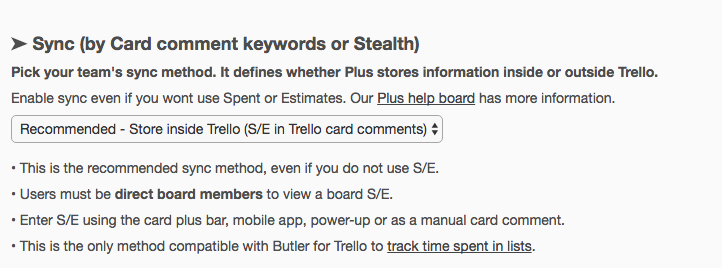
\includegraphics[width=\textwidth]{./afbeeldingen/synctrello.png}
	\caption{Instellen synchronisatie tijden in ``Plus For Trello''}
	\label{fig:synctrello}
\end{figure} 
\pagebreak
\paragraaf{Negatieve waarden voor R toelaten}
\noindent
\\Hoeveel tijd je nodig hebt om een taak af te ronden is niet makkelijk in te schatten.  Het kan dus gebeuren dat de geschatte tijd (E) lager ligt dan de effectief gepresteerde tijd (S). Hierdoor zal het aantal overgebleven uren (R) voor een kaart negatief uitvallen. Indien de optie in ``Plus For Trello'' niet geactiveerd is om negatieve uren toe te laten, zal automatisch het aantal E uren verhoogd worden als het aantal S uren boven die waarde  gaat. Hierdoor zal het aantal R uren nooit onder 0 komen te liggen. Dit is uiteraard geen juiste weergave van de verrichte prestaties, activeer daarom deze optie als volgt:
\begin{enumerate}[nolistsep]
	\item Klik op het zandloper icoontje van ``Plus for trello'' \korteverwijzing[fig:plusfortrello];
	\item Klik onder ``contents'' op ``Preferences'' en voer volgende instellingen uit \korteverwijzing[fig:prefsplusfortrello]
	\begin{itemize}
		\item Selecteer bij ``Work units'' de waarde ``hours'' indien nodig;
		\item Selecteer bij ``Week starts'' de waarde ``Monday'' indien nodig;
		\item Vink het vakje voor ``Allow negative Remaining (or never use Estimates).'' aan.
	\end{itemize}
\end{enumerate}

\begin{figure}[h]
	\centering
	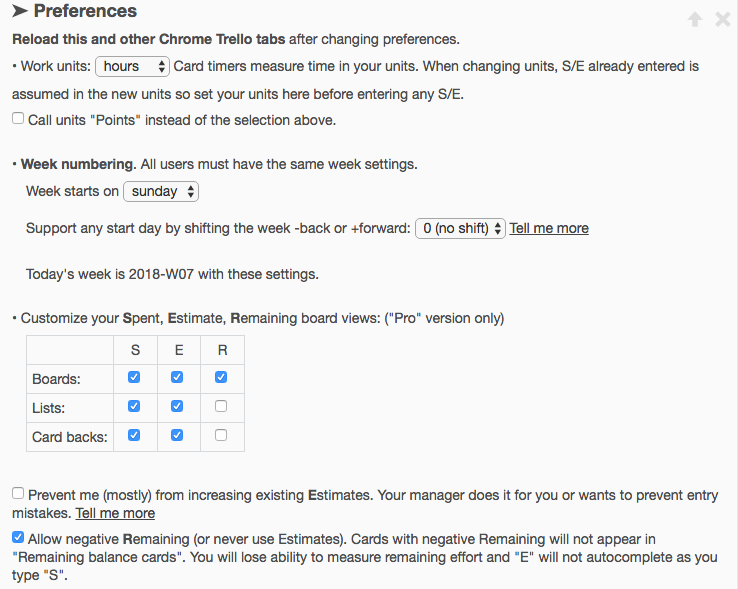
\includegraphics[width=\textwidth]{./afbeeldingen/prefsplusfortrello.png}
	\caption{Voorkeuren in ``Plus For Trello''}
	\label{fig:prefsplusfortrello}
\end{figure} 

\section{Overzicht}

Nadat je de invoegtoepassing heeft ge\"installeerd en bent aangemeld op de website krijg je een overzichtsscherm te zien met al jouw persoonlijke borden \korteverwijzing[fig:overzicht].

\begin{figure}[!h]
	\centering
	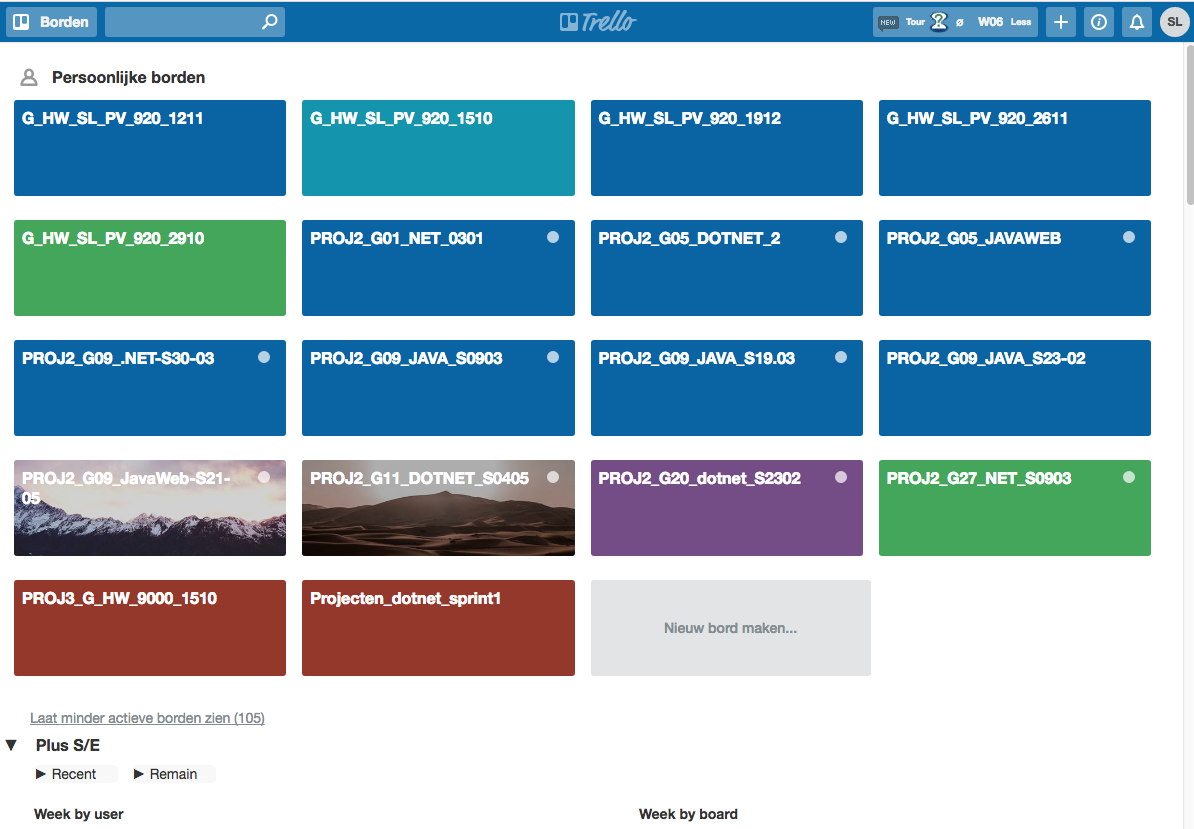
\includegraphics[width=\textwidth]{./afbeeldingen/overzicht.png}
	\caption{Hoofdscherm Trello}
	\label{fig:overzicht}	
\end{figure} 

\noindent
\\\\Volgende lijst toont een overzicht met functionaliteiten die overeenstemt met een nummer op figuur \ref{fig:overzicht_genummerd}. De belangrijkste functionaltieiten worden uitgebreid beschreven in deze handleiding.\\
\begin{enumerate}[nolistsep]
	\item Lijst borden
	\item Zoekfunctie
	\item Plus for Trello
	\item Aanmaken (Bord, team, bedrijfsteam) 
	\item Informatie
	\item Meldingen
	\item Account beheren
	\item Persoonlijke borden
	\item Nieuw bord maken
\end{enumerate}

\begin{figure}[!h]
	\centering
	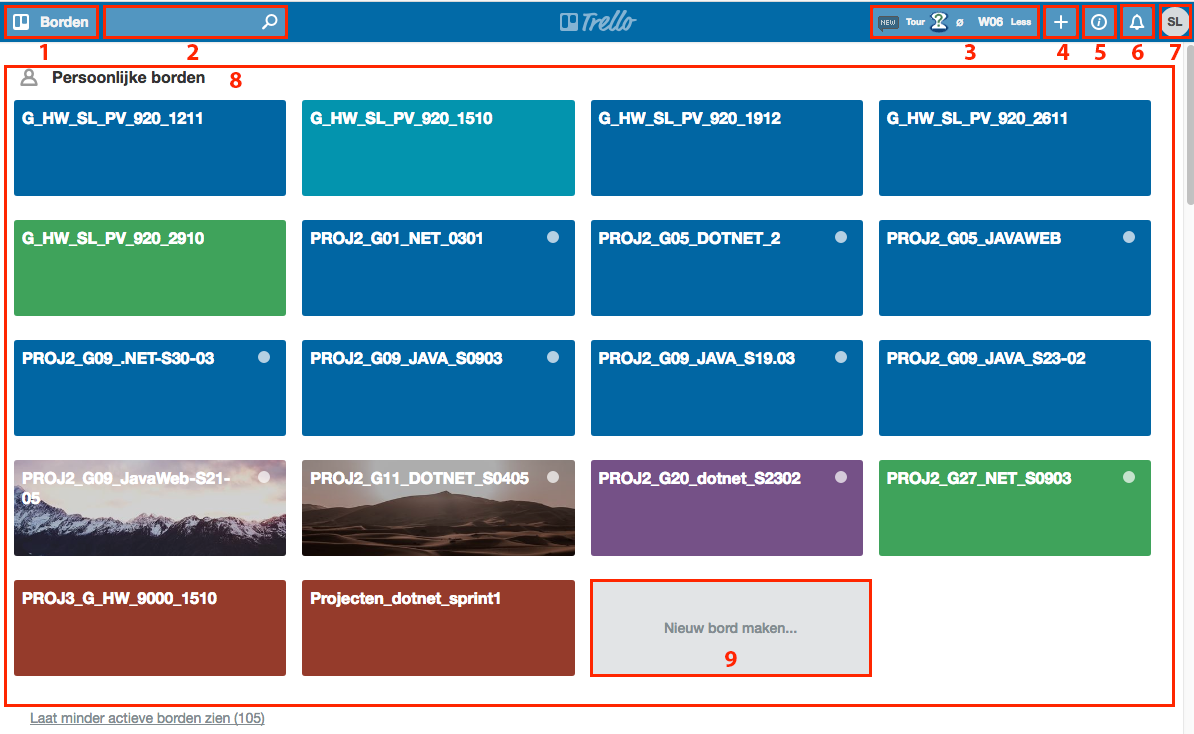
\includegraphics[width=\textwidth]{./afbeeldingen/overzicht_genummerd.png}
	\caption{Hoofdscherm Trello met aangeduide functionaliteit}
	\label{fig:overzicht_genummerd}	
\end{figure} 

\section{Stappenplan (Programmeren)}

Om snel met Trello aan de slag te kunnen gaan vind je hieronder een overzicht van stappen die voor elk project (Programmeren) moeten uitgevoerd worden in deze chronologische volgorde:
\begin{enumerate}[nolistsep]
	\item Maak jouw team aan voor het project dat bestaat uit jezelf en je groepsgenoten (Dit moet slechts door \'e\'en iemand gebeuren);
	\item Maak een nieuw bord aan met gewenste naamgeving voor jouw team;
	\item Voeg de betrokken lector(en) als lid (= Beheerder) toe aan jouw bord;
	\item Voeg lijsten toe op het bord (``Product backlog'', ``Sprint backlog'', ...);
	\item Voeg kaarten toe aan de lijst ``Product backlog'' OF kopieer de resterende kaarten uit deze lijst van een vorige sprint (bord);
	\item Verplaats de kaarten voor de huidige sprint naar ``Sprint backlog'' en voeg een inschatting (E uren) per teamlid toe aan elke verplaatste kaart;
	\item Voeg elke geleverde prestatie (S uren) per teamlid toe aan de bijhorende kaart;
	\item Verplaats een kaart indien zijn status wijzigt naar de bijhorende lijst;
	\item Herhaal stap 7-8 tijdens de huidige sprint;
	\item Ga terug naar stap 2 voor de volgende sprint.
\end{enumerate}

\section{Stappenplan (Systeembeheer)}

Om snel met Trello aan de slag te kunnen gaan vind je hieronder een overzicht van stappen die voor elk project (Systeembeheer) moeten uitgevoerd worden in deze chronologische volgorde:
\begin{enumerate}[nolistsep]
	\item Maak jouw team aan voor het project dat bestaat uit jezelf en je groepsgenoten (Dit moet slechts door \'e\'en iemand gebeuren);
	\item Maak een nieuw bord aan met gewenste naamgeving voor jouw team;
	\item Voeg de betrokken lector(en) als lid (= Beheerder) toe aan jouw bord;
	\item Voeg lijsten toe op het bord (``Backlog'', ``Ready'', ...);
	\item Voeg kaarten toe aan de lijst ``Backlog'';
	\item Verplaats een kaart van ``Backlog'' naar ``Ready'' en voeg een inschatting (E uren) per teamlid toe aan deze kaart;
	\item Voeg elke geleverde prestatie (S uren) per teamlid toe aan de bijhorende kaart;
	\item Verplaats een kaart indien zijn status wijzigt naar de bijhorende lijst;
	\item Herhaal stap 6-8 (ook 5 indien nodig) zolang het project loopt.
\end{enumerate}		
	\chapter{Team beheren}\label{chapter:team_beheren}

Indien je voor een project meerdere borden moet maken (zeker bij programmeren) is het aan te raden om eenmalig het team aan te maken. Zo moeten niet per bord steeds alle leden \'e\'en voor \'e\'en toegevoegd worden, maar kan je het team toevoegen.
\\\\
Het overzichtsscherm van een team \korteverwijzing[fig:overzicht_team] kan je bereiken door enerzijds in het hoofdscherm van Trello het team te kiezen, anderzijds kan je het scherm ook openen door op de teamnaam te klikken in een specifiek Trellobord van dat team en nadien ``Bekijk teampagina'' te selecteren.
\\
\begin{figure}[H]
	\centering
	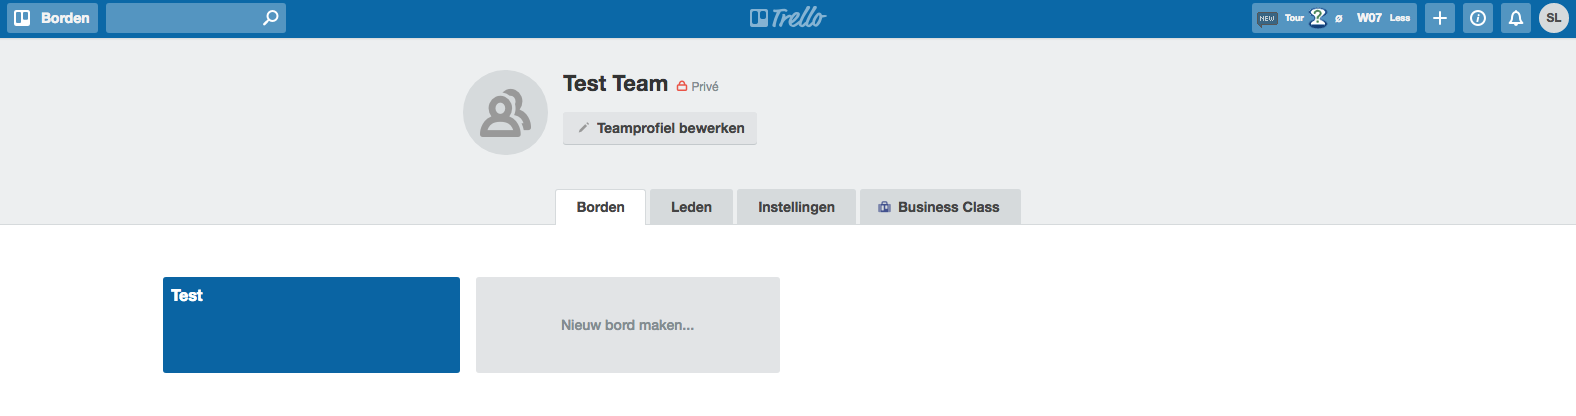
\includegraphics[width=\textwidth]{./afbeeldingen/overzicht_team.png}
	\caption{Overzichtscherm van een team}
	\label{fig:overzicht_team}	
\end{figure} 

\section{Team aanmaken}

Om een nieuw team aan te maken heb je de keuze uit deze 2 manieren:
\begin{itemize}
	\item Vanuit hoofdscherm Trello
	\begin{enumerate}[nolistsep]
		\item Scroll helemaal naar onder;
		\item Kies de optie ``Maak een nieuw team aan ...''.
	\end{enumerate}
\pagebreak
	\item Vanuit het detailscherm van hetTrellobord (van dat team)
	\begin{enumerate}[nolistsep]
		\item Klik op de teamnaam;
		\item Kies ``Wijzig team ...'' (Enkel als er al een team gekozen is anders vervalt deze stap);
		\item Kies ``Team cre\"eren.
	\end{enumerate}
\end{itemize}

\noindent
\\Vul daarna de gegevens aan \korteverwijzing[fig:aanmaken_team] en bevestig deze om het team effectief aan te maken. Nadien wordt het overzichtscherm van het team getoond \korteverwijzing[fig:overzicht_team]. Het is ook mogelijk om hier een nieuw bord aan te maken voor dat team.

\begin{figure}[H]
	\centering
	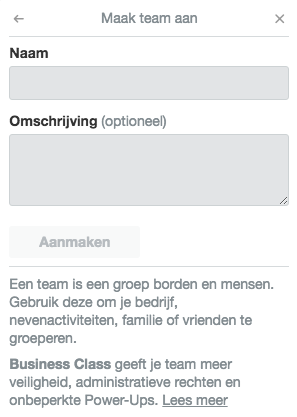
\includegraphics[scale=0.6]{./afbeeldingen/aanmaken_team.png}
	\caption{Aanmaken van een team}
	\label{fig:aanmaken_team}	
\end{figure} 

\section{Team wijzigen}

Om een team te wijzigen volstaat het om zijn overzichtspagina te openen van waaruit je toegang hebt tot volgende mogelijkheden:
\begin{itemize}
	\item Teamprofiel aanpassen;
	\item Leden toevoegen / verwijderen;
	\item Rechten van leden aanpassen;
	\item Teaminstellingen aanpassen.
\end{itemize}

\section{Team verwijderen}

Om een team te kunnen verwijderen voer je volgende stappen uit:
\begin{enumerate}[nolistsep]
	\item Open de teampagina;
	\item Selecteer ``instellingen'';
	\item Kies de optie ``Dit team verwijderen?'' onderaan de pagina;
	\item Bevestig het verwijderen.
\end{enumerate}

\noindent
\\Als je het team verwijdert van het huidige bord zal dit de waarde ``Persoonlijk'' voor zijn team krijgen.	
	\chapter{Bord beheren}

\section{Lijst van borden}

In het hoofdscherm \korteverwijzing[fig:overzicht] heb je in het midden van het scherm reeds een overzicht van jouw persoonlijke borden. Om een overzicht te krijgen van alle borden waartoe je toegang hebt maak je gebruik van de knop ``borden''  \korteverwijzing[fig:borden].
\\

\begin{figure}[h]
	\centering
	
\includegraphics[scale=.7]{./afbeeldingen/borden.png}
	\caption{Borden tonen}
	\label{fig:borden}	
\end{figure} 

\noindent
Eens je deze functionalteit geactiveerd hebt krijg je een lijst  \korteverwijzing[fig:lijst_borden] te zien met daarin alle borden waaraan je verbonden bent. Het is eveneens mogelijk om te zoeken naar een specifiek bord in deze lijst. Je kan dan het gewenste bord openen door dit te selecteren.\\

\begin{figure}[H]
	\centering
	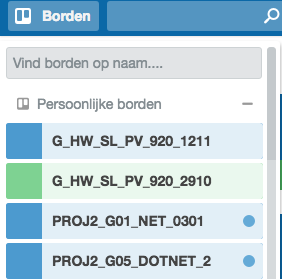
\includegraphics[scale=.5]{./afbeeldingen/lijst_borden.png}
	\caption{Voorbeeldlijst van al jouw borden}
	\label{fig:lijst_borden}	
\end{figure} 

\section{Bord aanmaken}

Een nieuw bord kan op twee manieren aamgemaakt worden:
\begin{enumerate}
	\item 
		\begin{enumerate}
			\item Activeer de ``+'' knop \korteverwijzing[fig:aanmaken_start];
			\item Selecteer nu ``Bord aanmaken'' \korteverwijzing[fig:aanmaken];
			\item Voer een naam in en kies het gewenste team \korteverwijzing[fig:nieuw_bord];
			\item Bevestig de ingevoerde waarden met ``aanmaken'' en het nieuwe Trellobord wordt aangemaakt en onmiddellijk geopend \korteverwijzing[fig:leeg_bord].
		\end{enumerate}
	\item 
		\begin{enumerate}
			\item Activeeer de ``Maak nieuw bord aan ...'' knop \korteverwijzing[fig:nieuw_bord_maken];
			\item Voer een naam in en kies het team \korteverwijzing[fig:nieuw_bord];
			\item Bevestig de ingevoerde waarden met ``aanmaken'' en het nieuwe Trellobord wordt aangemaakt en onmiddellijk geopend \korteverwijzing[fig:leeg_bord].
		\end{enumerate}
\end{enumerate}
\hfil
\begin{figure}[H]
	\centering
	\begin{subfigure}{.5\textwidth}
		\centering
		
\includegraphics[scale=1]{./afbeeldingen/plus.png}
		\captionof{figure}{Aanmaken}
		\label{fig:aanmaken_start}
	\end{subfigure}%
	\begin{subfigure}{.5\textwidth}
		\centering
		
\includegraphics[width=.9\textwidth]{./afbeeldingen/nieuw_bord_maken.png}
		\captionof{figure}{Nieuw bord maken ...}
		\label{fig:nieuw_bord_maken}
	\end{subfigure}\hfill
	\begin{subfigure}{.5\textwidth}
		\centering
		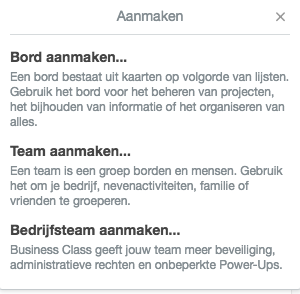
\includegraphics[width=\textwidth]{./afbeeldingen/aanmaken.png}
		\captionof{figure}{Aanmaken}
		\label{fig:aanmaken}
	\end{subfigure}%
	\begin{subfigure}{.5\textwidth}
		\centering
		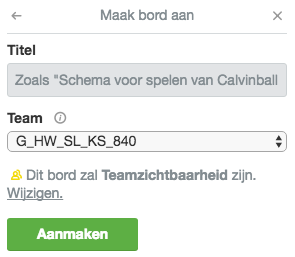
\includegraphics[width=\textwidth]{./afbeeldingen/nieuw_bord.png}
		\captionof{figure}{Nieuw bord}
		\label{fig:nieuw_bord}
	\end{subfigure}
	\caption{Aanmaken van een nieuw Trellobord}
	\label{fig:aanmaken_bord}
\end{figure}

\begin{figure}[H]
	\centering
	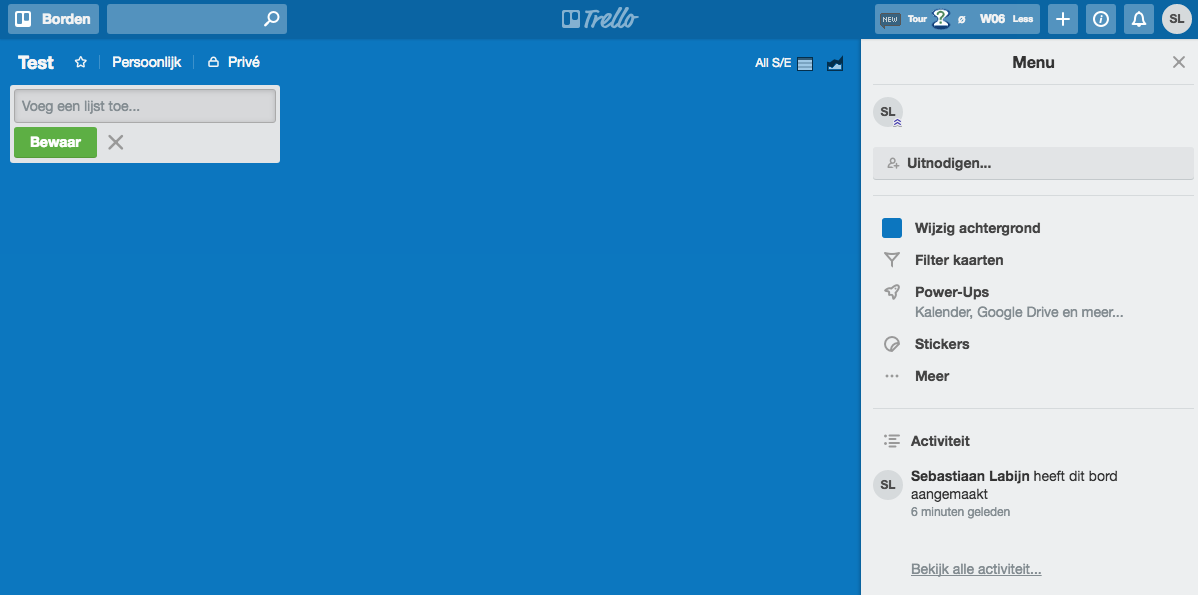
\includegraphics[width=\textwidth]{./afbeeldingen/leeg_bord.png}
	\caption{Een nieuw aangemaakt bord}
	\label{fig:leeg_bord}	
\end{figure} 

\section{Bord wijzigen}

Onderstaande lijst toont een overzicht met functionaliteiten \korteverwijzing[fig:leeg_bord_genummerd] om het bord te wijzigen die overeenstemmen met een nummer op die figuur. Deze worden uitgebreid beschreven in de volgende paragrafen.

\begin{enumerate}[nolistsep]
	\item Naam wijzigen;
	\item Team wijzigen;
	\item Zichtbaarheid aanpassen;
	\item Lijsten wijzigen \verwijzing[chapter:lijsten_beheren];
	\item Kaarten wijzigen \verwijzing[chapter:kaarten_beheren];
	\item Leden wijzigen  \verwijzing[chapter:leden_beheren];
	\item Weergave Trellobord aanpassen.
\end{enumerate}

\paragraaf{Naam wijzigen}
\noindent
\\Om de naam van het Trellobord te wijzigen onderneem je volgende stappen:
\begin{enumerate}[nolistsep]
	\item Selecteer de huidige naam;
	\item Voer de nieuwe naam in;
	\item Bevestig de wijziging.
\end{enumerate}	

\paragraaf{Team wijzigen}
\noindent
\\Selecteer het huidige team en kies daarna de gewenste waarde. Indien er nog geen team aan het bord gekoppeld is zie je de waarde ``Persoonlijk". Wanneer je een team kiest kan je extra opties voor dat team instellen \korteverwijzing[fig:wijzig_Team]. Als het team nog niet bestaat kan je via dit scherm ook de functionaliteit starten om het aan te maken \verwijzing[chapter:team_beheren].

\begin{figure}[H]
	\centering
	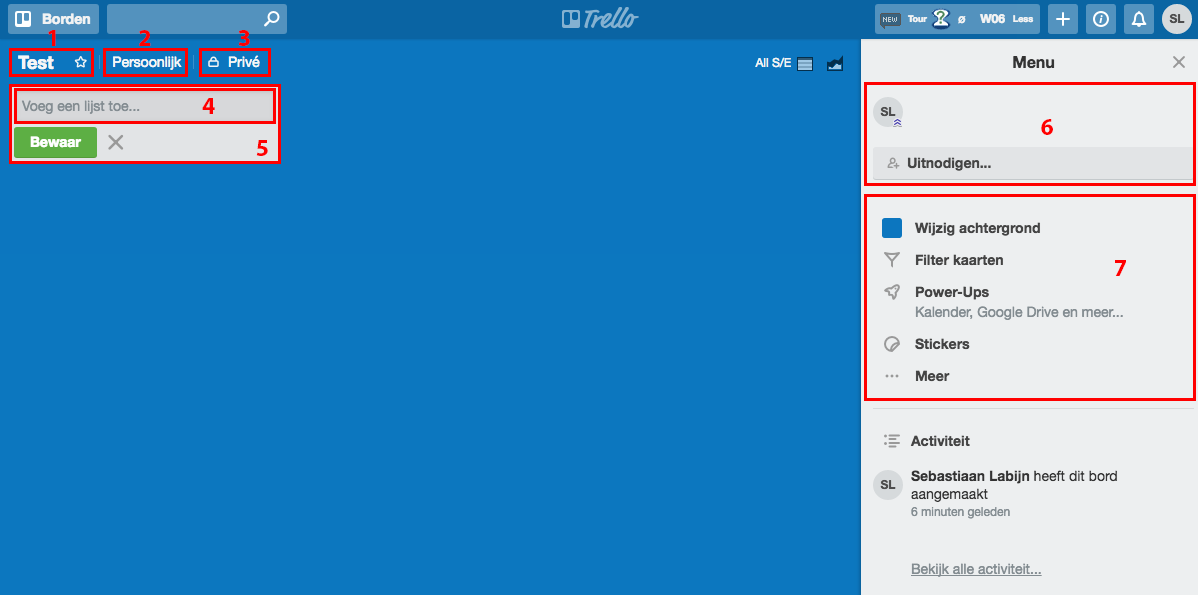
\includegraphics[width=\textwidth]{./afbeeldingen/leeg_bord_genummerd.png}
	\caption{Aanduiding belangrijkste functionaliteiten op een bord}
	\label{fig:leeg_bord_genummerd}	
\end{figure} 

\begin{figure}[H]
	\centering
	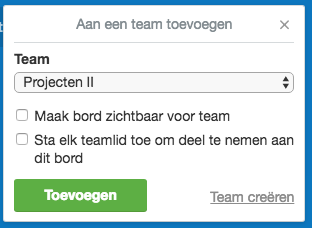
\includegraphics[scale=0.5]{./afbeeldingen/wijzig_team.png}
	\caption{Team wijzigen}
	\label{fig:wijzig_Team}	
\end{figure} 

\paragraaf{Zichtbaarheid aanpassen}
\noindent
\\Selecteer de huidige zichtbaarheid en kies daarna de gewenste zichtbaarheid. In Trello is er keuze uit drie verschillende modi:
\begin{itemize}
	\item Priv\'e: Enkel zichtbaar voor jou en de toegevoegde leden;
	\item Team: Enkel zichtbaar voor jou en de teamleden;
	\item Openbaar:  Zichtbaar voor iedereen die over de hyperlink naar het bord beschikt.
\end{itemize}	

\pagebreak

\paragraaf{Weergave bord aanpassen}
\noindent
\\Er is de mogelijkheid om onder andere volgende eigenschappen van het Trellobord aan te passen:
\begin{itemize}
	\item Achtergrond: Kies een achtergrondkleur of laad een foto op als achtergrond;
	\item Filter kaarten: Toon enkel kaarten die aan de filter voldoen;
	\item Power-ups: Integreer jouw Trellobord met tal van andere toepassingen (b.v.: Slack\footnote{\url{http://www.slack.com}}, GitHub\footnote{\url{http://www.github.com}});
	\item Stickers: Gebruik stickers.
\end{itemize}	
	\chapter{Lijsten beheren}\label{chapter:lijsten_beheren}

Aangezien er tijdens de projecten volgens het Agile principe wordt gewerkt is het nodig om de verschillende kaarten/taken te organiseren en deze onder te brengen in hun juiste status gedurende de iteratie. De status van een kaart/taak wordt bepaald door de lijst (kolom op het bord) waarin deze zich bevindt.

\noindent
\\Maak, per bord, lijsten aan die fasen voorstellen waarin elke taak zich zal bevinden. De naamgeving in het vet voor de / is voor programmeurs, de naamgeving in het cursief na de / is voor de systeembeheerders:
\begin{itemize}
	\item \textbf{Product Backlog} / \textit{Backlog}: Hierin komen alle kaarten die tijdens het volledige project nog moeten worden afgewerkt. Deze kolom bevat dus de resterende kaarten voor het project zelf en bevat kaarten over de borden heen. De kaarten zelf bevatten nog \textbf{geen} inschattingen;
	\item \textbf{Sprint Backlog} / \textit{Ready}: Dit is een lijst die alle kaarten bevat die op dit bord zullen worden uitgevoerd. Deze kaart wordt verplaatst vanuit de lijst ``Product backlog''. Tijdens het verplaatsen wordt ook de inschatting van de teamleden aan de kaart toegevoegd;
	\item \textbf{Doing} / \textit{Working}: Dit zijn kaarten waar het team momenteel effectief aan werkt;
	\item \textbf{Testing} / \textit{Testing}: Deze lijst bevat de kaarten die uitgevoerd zijn maar nog getest dienen te worden;
	\item \textbf{Done} / \textit{Ready for Review}: Dit zijn kaarten die volledig afgewerkt zijn.
\end{itemize}
Het is ook mogelijk om zelf nog extra lijsten toe te voegen. Indien een nieuw bord gemaakt wordt voor de volgende sprint wordt steeds de lijst ``product backlog'' integraal van het vorige bord overgenomen met behulp van ``Lijst kopi\"eren'' (Programmeren).

\section{Lijst aanmaken}
Om een lijst aan te maken onderneem je volgende stappen:
\begin{enumerate}[nolistsep]
	\item Selecteer het gewenste bord;
	\item Kies de optie ``Voeg een lijst toe...'';
	\item Voer de gewenste naam in;
	\item Kies ``Bewaar''.
\end{enumerate}

\section{Lijst wijzigen}
Er zijn verschillende wijzigingen die je aan een lijst kan aanbrengen.
\begin{itemize}
	\item Naam wijzigen
	\begin{enumerate}
		\item Klik op de naam van de lijst die je wenst te wijzigen;
		\item Voer de nieuwe naam in;
		\item Bevestig de wijzigingen.
	\end{enumerate}
	\item Plaats van de lijst wijzigen	
	\begin{enumerate}
		\item Selecteer de gewenste lijst;
		\item Sleep deze naar de gewenste plaats.
	\end{enumerate}
	\item Abonneren (Updates ontvangen indien lijst wijzigt)
	\begin{enumerate}
		\item Selecteer ``...'' op de gewenste lijst;
		\item Selecteer ``Abonneren''.
	\end{enumerate}
\end{itemize}
\noindent
\\Indien je een abonnement wil opzeggen voor een bepaalde lijst herhaal je gewoon de stappen voor ``Abonneren''.

\section{Lijst verplaatsen}

Het is ook mogelijk om een lijst en al zijn bijhorende kaarten te verplaatsen (zelfs naar een ander bord). Om dit te realiseren dienen volgende stappen uitgevoerd te worden:
\begin{enumerate}[nolistsep]
	\item Selecteer ``...'' op de gewenste lijst;
	\item Kies ``Verplaats lijst ..";
	\item Kies het gewenste ``bord'' en ``positie" (= kolomnummer) binnen dat bord;
	\item Bevestig met ``verplaats".
\end{enumerate}

\section{Lijst kopi\"eren}

Een lijst en al zijn bijhorende kaarten kunnen \textbf{binnen eenzelfde bord} op volgende manier gekopieerd worden:
\begin{enumerate}[nolistsep]
	\item Selecteer ``...'' op de gewenste lijst;
	\item Kies ``Kopieer lijst ..";
	\item Voer de gewenste ``naam'' in;
	\item Bevestig met ``maak een lijst aan".
\end{enumerate}

\section{Lijst verwijderen}

Om een lijst te verwijderen van een Trellobord dient de optie ``lijst archiveren'' geactiveerd te worden. Deze is te bereiken via de optie ``...'' bij de gewenste lijst en dan ``Archiveer lijst''.\\
 \textbf{AANDACHT:} Trello vraagt niet om een bevestiging, dus de lijst en al zijn bijhorende kaarten zijn onmiddellijk verwijderd!	
	\chapter{Kaarten beheren}\label{chapter:kaarten_beheren}

Om de opvolging van een project te kunnen garanderen moet elk teamlid kunnen aantonen welke prestaties hij geleverd heeft. Hiervoor zullen er kaarten aan het bord toegevoegd worden. Een kaart staat dan voor een taak waaraan \'e\'en of meerdere teamleden zullen werken. Op elke kaart wordt een individuele inschatting toegevoegd wanneer deze uit de ``Product backlog'' (of ``Backlog'') verplaatst wordt en nadien wordt ook elke prestatie voor deze kaart geleverd hier gelogd. Zo krijgen we nadien een overzicht of het aantal gepresteerde uren in lijn ligt met de oorspronkelijke inschatting.

\section{Kaart toevoegen}

Om een kaart aan te maken dien je volgende stappen te ondernemen:
\begin{enumerate}[nolistsep]
	\item Kies de gewenste lijst;
	\item Kies ``Een kaart toevoegen ...'';
	\item Voer de gewenste omschrijving in;
	\item Maak de kaart aan met ``Voeg toe''.
\end{enumerate}

\noindent
\\De nieuwe kaart is dan toegevoegd aan de gekozen lijst \korteverwijzing[fig:nieuwe_kaart]

\begin{figure}[h]
	\centering
	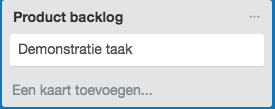
\includegraphics[scale=0.5]{./afbeeldingen/nieuwe_kaart.png}
	\caption{Voorbeeld nieuwe kaart}
	\label{fig:nieuwe_kaart}	
\end{figure} 

\section{Kaart wijzigen}

Een lege kaart zegt uiteraard niet zo veel op ons Trellobord dus deze kan op volgende manieren aangepast worden:
\begin{enumerate}[nolistsep]
	\item Naam wijzigen;
	\item Leden wijzigen;
	\item Labels beheren;
	\item Checklist beheren;
	\item Bijlage(s) beheren;
	\item Tijdsbesteding beheren \verwijzing[section:tijdsbesteding];
	\item Kaart verplaatsen, kopi\"eren of archiveren \verwijzing[chapter:kaarten_beheren].
\end{enumerate}

\noindent
\\Alle bovenstaande functionaliteiten worden toegelicht vanuit het detailscherm van een kaart \korteverwijzing[fig:detail_kaart]. Om het detailscherm van een kaart te openen volstaat het om op de kaart te ``klikken'' op het overzichtscherm van het Trellobord.

\begin{figure}[H]
	\centering
	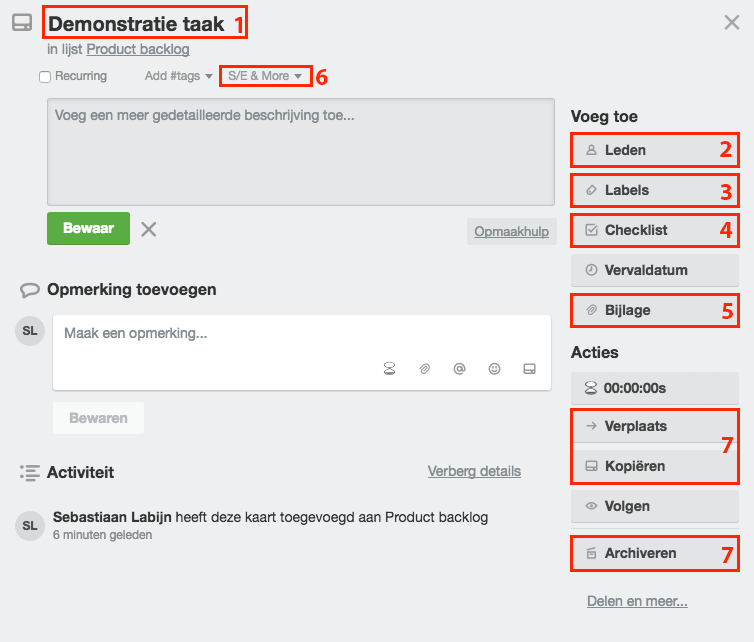
\includegraphics[scale=0.5]{./afbeeldingen/detail_kaart_genummerd.png}
	\caption{Detailscherm kaart met nummering functionaliteiten}
	\label{fig:detail_kaart}	
\end{figure} 

\paragraaf{Naam wijzigen}
\noindent
\\
Om de naam te wijzigen van een kaart kan men enerzijds in het overzichtscherm van het Trellobord op de naam klikken en deze dan aanpassen. Anderzijds kan men ook de naam aanpassen in het detailscherm op eenzelfde manier.

\paragraaf{Leden wijzigen}\label{paragraaf:leden_wijzigen}
\noindent
\\Het is soms nodig om per kaart de leden te kunnen beheren. Via deze weg kunnen we dan ook leden aan de kaart toevoegen of verwijderen zonder dat dit impact heeft op de rest van het bord. Om dit te verwezenlijken selecteer je ``leden'' en zoek dan het gewenste lid om dit toe te voegen of te verwijderen \korteverwijzing[fig:beheer_leden_kaart]

\begin{figure}[H]
	\centering
	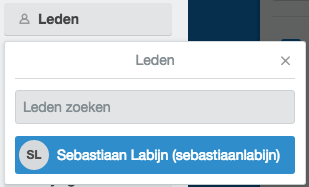
\includegraphics[scale=0.4]{./afbeeldingen/beheer_leden_kaart.png}
	\caption{Leden toevoegen/verwijderen op kaart}
	\label{fig:beheer_leden_kaart}	
\end{figure} 

\paragraaf{Labels beheren}
\noindent
\\
Om snel een overzicht te krijgen in de kaarten op een bord is het van groot belang om met labels te werken. Labels zijn kleurcodes die structuur aanbrengen in de aanwezige kaarten. Zo is het bij voorbeeld mogelijk om alle kaarten met ``geel'' te markeren die te maken hebben met een databank, alles met ``rood'' voor web, ... Op die manier kan het team snel zien welk type van kaarten er nog moeten behandeld worden of welke er allemaal afgewerkt zijn.

\noindent
\\Om een label aan kaart toe te voegen selecteer je ``labels'' en daarna kies je de gewenste kleur van het label. Het is ook mogelijk om een kleur een omschrijving te geven. Selecteer hiervoor het ``potlood'' naast de gewenste kleur. Daarnaast kan ook een nieuw label aangemaakt worden met een eigen kleur via ``Maak nieuw label aan...'' \korteverwijzing[fig:maak_label_aan]. Het gekozen label wordt dan weergegeven in het detailoverzicht van het scherm \korteverwijzing[fig:detail_kaart_labels]. Door op het labelkleur te klikken in het detailoverzicht kan je een label ook terug verwijderen van een kaart. De labels op een kaart worden ook getoond op de kaart in het Trellobord zelf \korteverwijzing[fig:bord_checklist]. Zo heb je snel een overzicht op je bord welke kaarten met welk label verbonden zijn.

\begin{figure}[H]
	\centering
	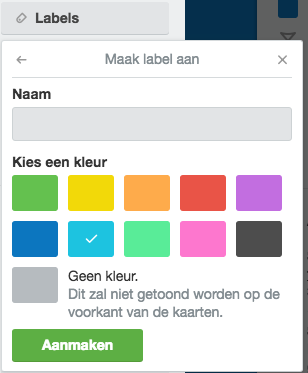
\includegraphics[scale=0.6]{./afbeeldingen/maak_label_aan.png}
	\caption{Labels aanmaken}
	\label{fig:maak_label_aan}	
\end{figure} 

\begin{figure}[H]
	\centering
	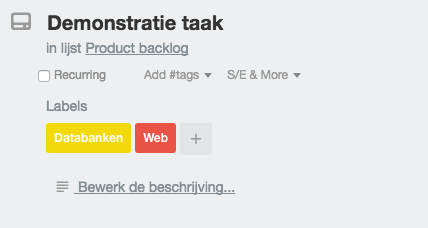
\includegraphics[scale=0.5]{./afbeeldingen/detail_kaart_labels.png}
	\caption{Kaart met labels}
	\label{fig:detail_kaart_labels}	
\end{figure} 

\paragraaf{Checklist beheren}
\noindent
\\
Checklists zijn zeer handig als een kaart uit meerdere onafhankelijke deeltaken bestaat zodat ook de voortgang binnen een kaart kan opgevolgd worden. Om een checklist toe te voegen kies je ``Checklist'' in het menu en voer dan de naam in voor de checklist. Indien er al een checklist aangemaakt was kan je hier ook keizen om items uit een vorige checklist mee te kopi\"eren. De nieuwe checklist verschijnt na bevestiging in het detailoverzicht van de kaart \korteverwijzing[fig:nieuwe_checklist].

\begin{figure}[H]
	\centering
	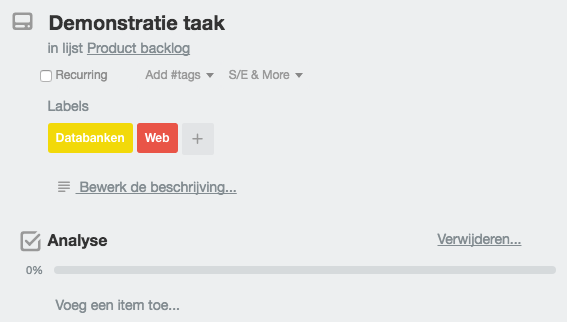
\includegraphics[scale=0.5]{./afbeeldingen/nieuwe_checklist.png}
	\caption{Kaart met lege checklist}
	\label{fig:nieuwe_checklist}	
\end{figure} 

\noindent
\\Nadien kan je in het detailzicht van de kaart ook items toevoegen aan de checklist zodat de individuele werkpunten zichtbaar worden \korteverwijzing[fig:checklist_items].

\begin{figure}[H]
	\centering
	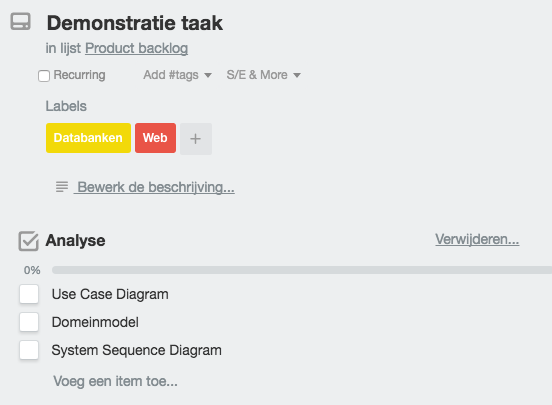
\includegraphics[scale=0.5]{./afbeeldingen/checklist_items.png}
	\caption{Checlist met items}
	\label{fig:checklist_items}	
\end{figure} 

\noindent
\\Het voordeel hiervan is dat deze voortgang ook getoond wordt op het algemene Trellobord \korteverwijzing[fig:bord_checklist]. Hierdoor hoeft het team niet telkens een kaart te openen om de voortgang te kunnen raadplegen, maar is alles snel vanuit het hoofdoverzicht te bekijken.

\begin{figure}[H]
	\centering
	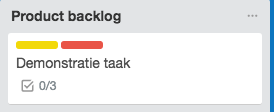
\includegraphics[scale=0.75]{./afbeeldingen/bord_checklist.png}
	\caption{Trellobord met kaart met checklist}
	\label{fig:bord_checklist}	
\end{figure} 

\paragraaf{Bijlages beheren}
\noindent
\\Bijlages kunnen een schat aan informatie zijn voor een team bij een bepaalde kaart. Deze kunnen bij voorbeeld mock-ups zijn van de layout, documenten van de opdrachtgever, gesprekken via Slack, GitHub requests... Het is dan ook heel belangrijk dat de bijlages op kaarten op een goede manier beheerd worden.
\noindent
\\\\Een nieuwe bijlage kan toegevoegd worden vanuit het detailscherm van een kaart. Hierbij kan je kiezen uit verschillende soorten bestanden:
\begin{itemize}
	\item Lokaal bestand;
	\item Trellobord of -kaart;
	\item Cloud Bestand (DropBox\footnote{\url{https://www.dropbox.com}}, Google Drive\footnote{\url{https://www.google.be/drive/about.html}}, OneDrive \footnote{\url{https://www.onedrive.com}}, ... );
	\item Hyperlink.
\end{itemize}
\noindent
De toegevoegde bijlages zijn dan ook zichtbaar in het detailzicht van de kaart \korteverwijzing[fig:bijlage_kaart]. Het is ook hier dat je bijlages kan verwijderen en eventueel extra bijlages toevoegen. Een bijlage raadplegen kan door deze aan te klikken of het bestand, indien mogelijk, te downloaden. Het is echter niet mogelijk om een bijlage aan te passen. Indien dit toch gewenst is moet de bijlage eerst verwijdert worden om ze nadien aangepast toe te voegen.

\begin{figure}[H]
	\centering
	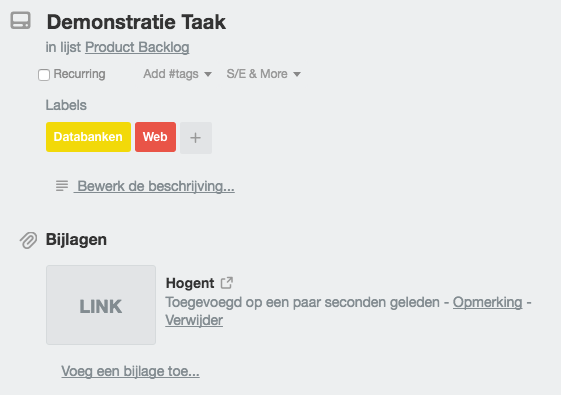
\includegraphics[scale=0.5]{./afbeeldingen/bijlage_kaart.png}
	\caption{Detailzicht van kaart met bijlage}
	\label{fig:bijlage_kaart}	
\end{figure} 

\section{Kaart(en) kopi\"eren}

Om een kaart te kopi\"eren onderneem je volgende stappen:
\begin{enumerate}[nolistsep]
	\item Open het detailzicht voor de gewenste kaart;
	\item Kies ``Kopieer'' onder ``Acties'';
	\item Kies de juiste instellingen \korteverwijzing[fig:kopieer_kaart];
	\item Bevestig met ``Kaart aanmaken''.
\end{enumerate}

\begin{figure}[H]
	\centering
	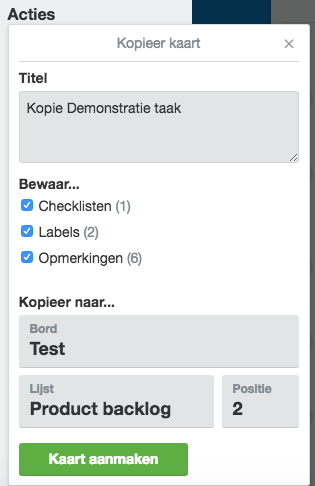
\includegraphics[scale=0.45]{./afbeeldingen/kopieer_kaart.png}
	\caption{Opties bij kopi\"eren van een kaart}
	\label{fig:kopieer_kaart}	
\end{figure} 
\noindent
\\Wil je meerdere kaarten tegelijk kop\"ieren? Herhaal dan bovenstaande stap voor elke kaart. Indien alle kaarten op een lijst moeten gekopieerd worden is het beter om de lijst zelf te kopi\"eren \verwijzing[chapter:lijsten_beheren]. 

\section{Kaart(en) verplaatsen}

Een kaart verplaatsen kan op verschillende manieren:
\begin{itemize}
	\item Wisselen van positie op eenzelfde lijst;
	\item Naar een andere lijst verplaatsen;
	\item Naar een lijst op een ander bord verplaatsen.
\end{itemize} 
\noindent
De eerste twee manieren kan je, naast de algemene methode hierna beschreven, ook verwezenlijken door de gewenste kaart vanuit het hoofdzicht van het Trellobord te verslepen naar de gewenste plaats. Wil je echter een kaart naar een ander bord verplaatsen dan kan dat enkel op de volgende manier:
\begin{enumerate}[nolistsep]
	\item Open het detailzicht voor de gewenste kaart;
	\item Kies ``Verplaatsen'' onder ``Acties'';
	\item Selecteer het gewesnte ``bord'', ``lijst'' en ``positie'' \korteverwijzing[fig:verplaats_kaart];
	\item Na bevestiging met `Verplaats'' is de kaart naar de gewenste plaats verschoven.
\end{enumerate}

\begin{figure}[h]
	\centering
	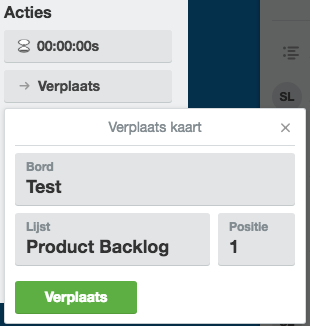
\includegraphics[scale=0.6]{./afbeeldingen/verplaats_kaart.png}
	\caption{Opties bij verplaatsen van een kaart}
	\label{fig:verplaats_kaart}	
\end{figure} 
\noindent
\\\\Om meerdere kaarten tegelijk te verplaatsen moet je bovenstaande stap voor elke te verplaatsen kaart herhalen.

\section{Kaart(en) verwijderen}

Een kaart verwijderen komt, net zoals bij lijsten, neer op het archiveren van de kaart. Om een kaart effectief van het bord te verwijderen onderneem je volgende stappen:
\begin{enumerate}[nolistsep]
	\item Open het detailzicht voor de gewenste kaart;
	\item Kies ``Archiveren'' onder ``Acties'';
	\item De kaart is nu gearchiveerd \korteverwijzing[fig:archiveer_kaart];
	\item Om de kaart definitief te verwijderen kies ``- verwijder'' OF kies ``\CircleArrowleft  Verstuur naar bord'' om archivatie ongedaan te maken;
	\item Na bevestiging is de kaart verdwenen van het bord OF teruggeplaatst op het bord.
\end{enumerate}

\begin{figure}[h]
	\centering
	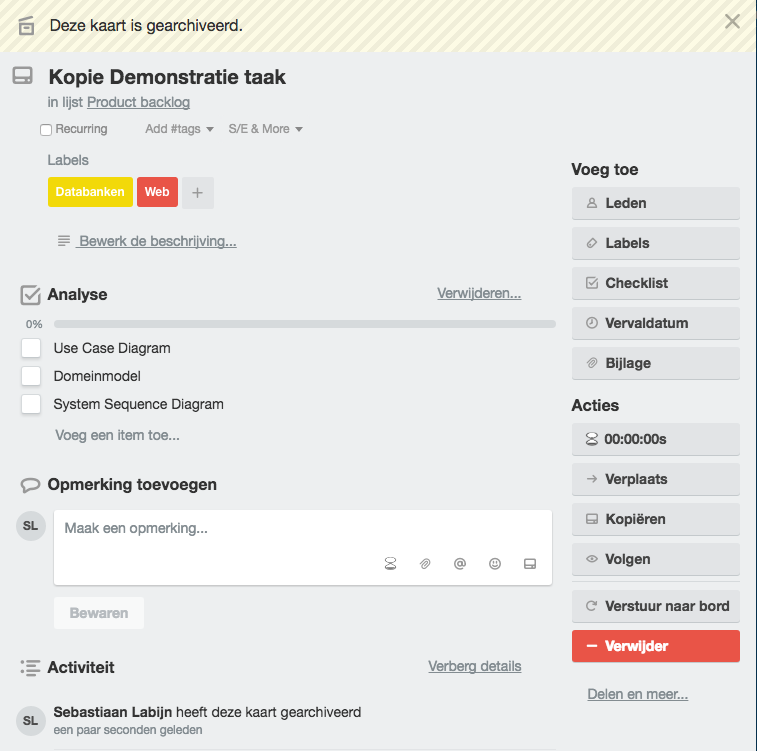
\includegraphics[scale=0.5]{./afbeeldingen/archiveer_kaart.png}
	\caption{Een gearchiveerde kaart}
	\label{fig:archiveer_kaart}	
\end{figure} 
\noindent
\\\\Om meerdere kaarten tegelijk te verwijderen moet je bovenstaande stap voor elke te verwijderen kaart herhalen.
Als je alle kaarten op een lijst wilt verwijderen is het veel effici\"enter om de lijst zelf te verwijderen \verwijzing[chapter:lijsten_beheren].

\section{Tijdsbesteding beheren}\label{section:tijdsbesteding}

Kaarten alleen op een lijst zeggen niet alles. Daarom is het van groot belang om ook de inschatting(en) en prestatie(s) te koppelen aan de juiste taken. Om dit te doen moeten de uren per teamlid toegevoegd worden op de bijhorende kaart(en). 
%De tijdsregistratie kan op twee manieren gebeuren: manueel of geautomatiseerd. \textbf{AANDACHT:} je kan enkel S uren geautomatiseerd toevoegen! Alle andere bewerkingen verlopen steeds volgens de manuele manier.

% titel in commentaar omdat geautomatiseerde methode weg(in commentaar) is
%\subsection{Manuele registratie}

\paragraaf{Toevoegen}
\\
Om de tijdseenheden toe te voegen volstaat het om volgende stappen uit te voeren:
\begin{enumerate}[nolistsep]
	\item Kies de gewenste kaart;
	\item Open het detailzicht van de kaart;
	\item Open het menu ``S/E \& more'';
	\item Kies de optie ``Add Spent' of ``Add Estimate'' afhankelijk van welke uren moeten gelogd worden;
	\item Vul de juiste waarden in voor ``S'', ``E'' en omschrijving \korteverwijzing[fig:aanmaken_prestatie];
	\item Bevestig de ingevulde uren via ``enter''.
\end{enumerate}

\begin{figure}[H]
	\centering
	
\includegraphics[scale=0.5]{./afbeeldingen/aanmaken_prestatie.png}
	\caption{Aanmaken inschatting/prestatie op een kaaart}
	\label{fig:aanmaken_prestatie}	
\end{figure} 

\noindent
\\Er werd een rij met ingevoerde uren toegevoegd \korteverwijzing[fig:aangemaakte_prestatie].
\\ \textbf{AANDACHT:} eens een rij is aangemaakt is, kan je deze NIET meer verwijderen, enkel aanpassen!

\begin{figure}[H]
	\centering
	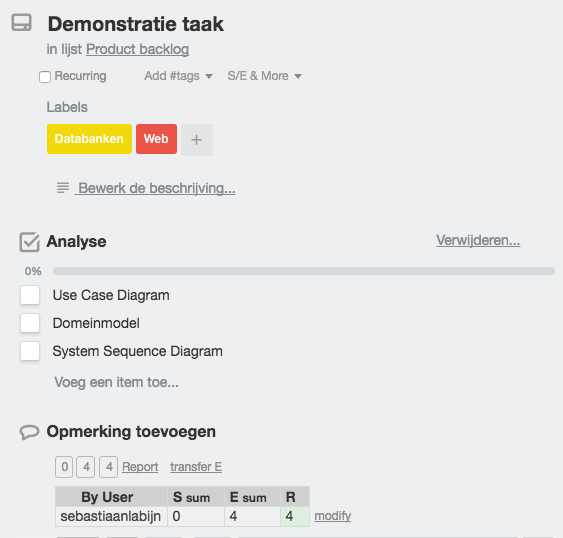
\includegraphics[scale=0.4]{./afbeeldingen/aangemaakte_prestatie.png}
	\caption{Kaart met een nieuwe inschatting}
	\label{fig:aangemaakte_prestatie}	
\end{figure} 

\paragraaf{Aanpassen}
\\
Om de tijdseenheden aan te passen volstaat het om volgende stappen uit te voeren:
\begin{enumerate}[nolistsep]
	\item Kies de gewenste kaart;
	\item Open het detailzicht van de kaart;
	\item Zoek de rij met uren die aangepast moeten worden;
	\item Selecteer ``modify'';
	\item Vul de juiste waarden in voor ``S'', ``E'' en voeg de reden van aanpassen toe indien nodig \korteverwijzing[fig:wijzigen_prestatie]
	\item Bevestig de wijziging met ``modify''
\end{enumerate}

\begin{figure}[H]
	\centering
	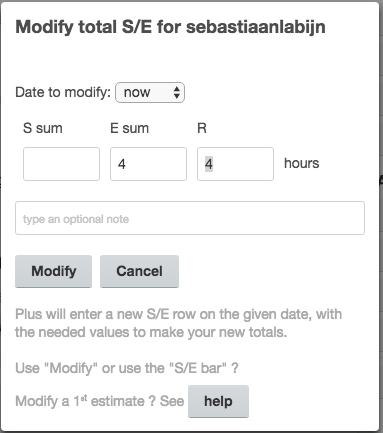
\includegraphics[scale=0.35]{./afbeeldingen/wijzigen_prestatie.png}
	\caption{Aanpassen tijdsbesteding op een kaaart}
	\label{fig:wijzigen_prestatie}	
\end{figure} 

\noindent
\\De uren op de gekozen rij werden aangepast \korteverwijzing[fig:gewijzigde_prestatie].

\begin{figure}[h]
	\centering
	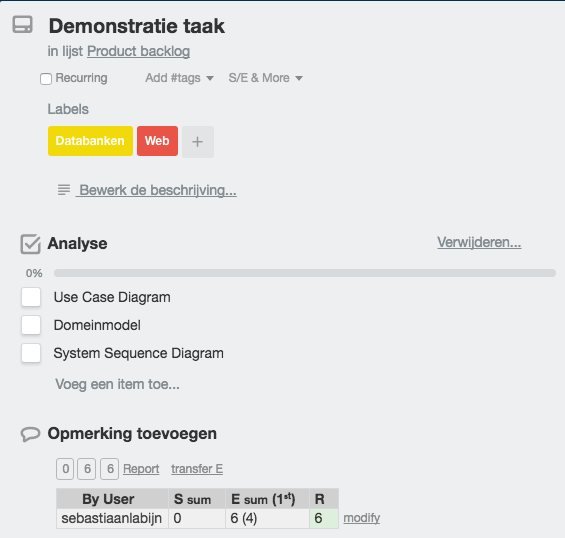
\includegraphics[scale=0.5]{./afbeeldingen/gewijzigde_prestatie.png}
	\caption{Kaart met een gewijzigde tijdsbesteding}
	\label{fig:gewijzigde_prestatie}	
\end{figure} 

\paragraaf{Uitwisselen inschatting}
\\
De techniek om uren uit te wisselen wordt vooral gebruikt indien de inschatting van de kaart niet invidueel maar op teamniveau gebeurt. De E uren worden dan toegekend aan het teamlid ``global''. Als een teamlid dan aan een kaart zal werken, transfereert hij eerst E uren van ``global'' naar zichzelf. Deze techniek kan ook gebruikt worden om tussen teamleden onderling E uren uit te wisselen. Dit doen we op een volgende manier:
\begin{enumerate}[nolistsep]
	\item Open het detailzicht van de kaart;
	\item Open het menu ``Transfer Estimate'';
	\item Voer volgende acties uit in het uitwisselscherm \korteverwijzing[fig:overzetten_prestatie]:
		\begin{enumerate}[nolistsep]
			\item ``From'': Teamlid van wie de uren overgeplaatst worden; 
			\item ``To'': Teamlid dat de uren ontvangt; 
			\item Vul het gewenste aantal E uren in;
			\item De nieuwe situatie wordt onmiddellijk in de tabel onderaan weergegeven.
		\end{enumerate}
	\item Bevestig de overplaatsing met ``enter''.
\end{enumerate}

\begin{figure}[h]
	\centering
	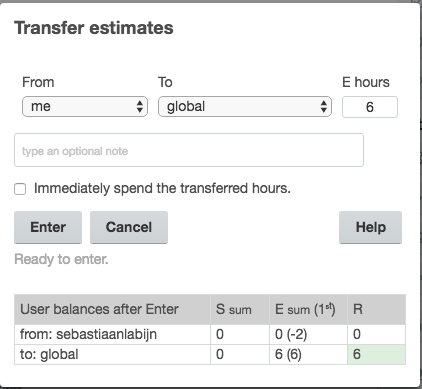
\includegraphics[scale=0.55]{./afbeeldingen/overzetten_prestatie.png}
	\caption{Overplaatsen inschatting op een kaart}
	\label{fig:overzetten_prestatie}	
\end{figure} 

\noindent
\\De uren zijn nu uitgewisseld tussen de twee teamleden \korteverwijzing[fig:overgezette_prestatie].

\begin{figure}[h]
	\centering
	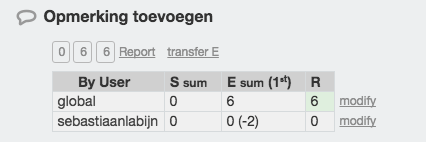
\includegraphics[scale=0.55]{./afbeeldingen/overgezette_prestatie.png}
	\caption{Kaart met een overgeplaatste prestatie}
	\label{fig:overgezette_prestatie}	
\end{figure} 

\begin{comment}
\subsection{Geautomatiseerde registratie}

Het is ook mogelijk om Trello een prestatie (ENKEL S uren) ``automatisch'' te laten registeren op een kaart. Dit gebeurt door de zandloper op de kaart, in zijn detailzicht onder acties, te activeren \korteverwijzing[fig:start_auto_reg]. 

\begin{figure}[H]
	\centering
	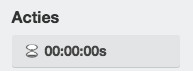
\includegraphics[scale=0.5]{./afbeeldingen/start_auto_reg.png}
	\caption{Start automatische registratie voor een prestatie}
	\label{fig:start_auto_reg}	
\end{figure} 

\noindent
\\De klok begint nu te lopen en \textbf{MOET} ook terug ``manueel'' stopgezet worden om de prestatie te be\"eindigen en nadien moet je de taak bevestigen alvorens ze effectief aan de kaart wordt toevoegd \korteverwijzing[fig:start_auto_reg]. De klok wordt dan al terug op 0 geplaatst.

\begin{figure}[H]
	\centering
	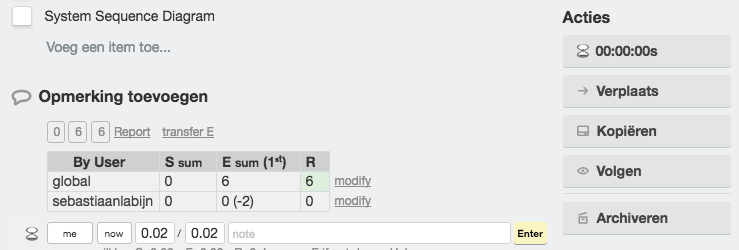
\includegraphics[scale=0.5]{./afbeeldingen/stop_auto_reg.png}
	\caption{Bevestigen automatische registratie voor een prestatie}
	\label{fig:stop_auto_reg}	
\end{figure} 
\noindent
\textbf{AANDACHT:} De browser afsluiten zal de klok NIET automatisch stopzetten! Zolang de klok loopt heb je in Chrome ook een extra venster dat je herrinnert aan de timer \korteverwijzing[fig:tijdens_auto_reg].

\begin{figure}[H]
	\centering
	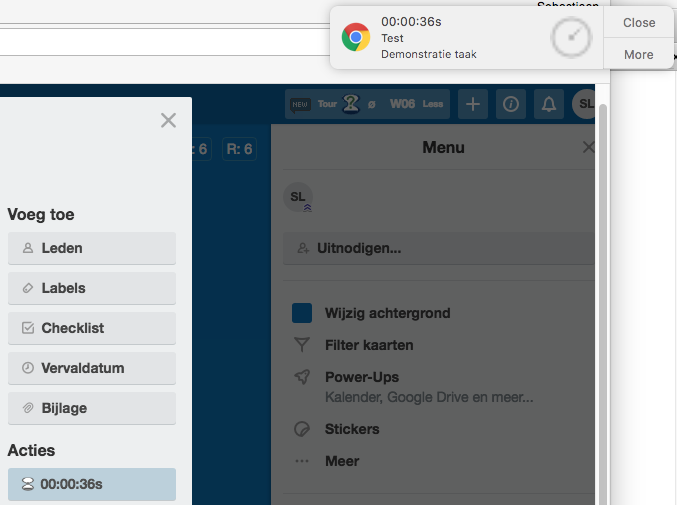
\includegraphics[scale=0.5]{./afbeeldingen/tijdens_auto_reg.png}
	\caption{Kaart tijdens automatische registratie voor een prestatie}
	\label{fig:tijdens_auto_reg}	
\end{figure} 

\noindent
\\Na bevestiging werd de prestatie aan de kaart toegevoegd \korteverwijzing[fig:prestatie_auto_reg]. Deze prestatie ziet er net uit als een manuele registratie dus er is geen onderscheid tussen beiden. Gebruik deze optie dus enkel en alleen voor kleine taken zodat je de timer zeker niet vergeet stop te zetten. Indien dit toch zo was zal je prestatie manueel moeten aanpassen, zoals reeds hiervoor beschreven.

\begin{figure}[h]
	\centering
	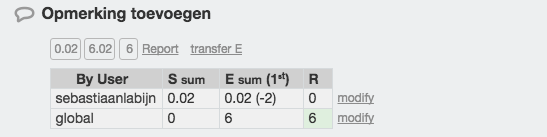
\includegraphics[scale=0.5]{./afbeeldingen/prestatie_auto_reg.png}
	\caption{Kaart met een automatische registratie voor een prestatie}
	\label{fig:prestatie_auto_reg}	
\end{figure} 
\end{comment}	
	\chapter{Leden beheren}\label{chapter:leden_beheren}

\section{Leden toevoegen}

Een lid kan op twee niveaus toevoegd worden in Trello. Enerzijds kan een lid aan het bord toevoegd worden maar het is ook mogelijk om een lid aan een individuele kaart toe te voegen \verwijzing[chapter:kaarten_beheren]. 
\noindent
\\\\Om een lid aan een bord toe voegen gebruik je de optie ``Uitnodigen ...'' in het detailzicht van het Trellobord. Zoek daarna de gewenste persoon en nodig hem uit voor jouw bord.

\section{Ledenstatus wijzigen}

In Trello kan heeft een lid van een bord twee mogelijke statussen:
\begin{itemize}
	\item Beheerder: Kan kaarten bekijken en bewerken, leden verwijderen en alle bordinstellingen wijzigen.
	\item Normaal: Kan kaarten bekijken en bewerken. Kan enkele bordinstellingen wijzigen.
\end{itemize}
\noindent
\\Om de status van een lid te wijzigen op jouw bord volstaat het om het icoon van het lid te klikken onder ``menu'' rechts op het hoofdschem van het Trellobord en nadien ``Wijzig rechten ...'' te kiezen.

\section{Leden verwijderen}

Om een lid van een bord te verwijderen selecteer je het icoon van het lid door te klikken onder ``menu'' rechts op het hoofdschem van het Trellobord en nadien ``Verwijder van bord ...'' te kiezen. Na bevestiging is het lid effectief van het bord verwijderd.	
	\chapter{Statistieken}

Via de invoegtoepassing ``Plus for Trello'' is het mogelijk om tal van rapporten te genereren die toelaten om de werking van het project en zijn team te analyseren. We beperken ons in deze handleiding tot de beschrijving van de belangrijkste statistieken.

\section{Overzicht algemene tijdsbesteding}

Dankzij ``Plus for Trello'' is er steeds een algemeen overzicht van de tijdsbesteding te raadplegen in het detailscherm van het Trellobord \korteverwijzing[fig:stats]. In dit overzicht zijn drie verschillende tijdseenheden te zien:
\begin{itemize}
	\item S: Spent, dit de som van uren die de leden gespendeerd hebben op het bord;
	\item E : Estimate, dit is het totaal van alle ingeschatte uren voor de kaarten op het bord;
	\item R : Remaining, verschil van E en S. Dit zijn het aantal resterende uren dat het team nog heeft om aan kaarten op dit bord te werken.
\end{itemize}
Het is mogelijk om deze tijdseenheden te baseren op een andere eenheid dan ``uur'' (bij voorbeeld: minunten of punten). De voorkeur is echter om steeds ``uur'' als tijdseenheid te hanteren.
\begin{figure}
	\centering
	
\includegraphics[scale=0.75]{./afbeeldingen/stats.png}
	\caption{Overzicht tijdsbesteding}
	\label{fig:stats}	
\end{figure} 

\section{Overzicht invididuele tijdsbesteding}

Om de S, E en R uren meer in detail te kunnen anyseren is er de mogelijkheid om een lijst te raadplegen \korteverwijzing[fig:individueleprestatiesknop]. 
\begin{figure}[H]
	\centering
	
\includegraphics[scale=0.75]{./afbeeldingen/individueleprestatiesknop.png}
	\caption{Genereren lijst individuele prestaties}
	\label{fig:individueleprestatiesknop}	
\end{figure} 
\noindent
Hier vinden we een overzicht van alle geleverde (= geregistreerde) prestaties op dit bord opgedeeld per kaart. In dit overzicht \korteverwijzing[fig:individueleprestaties] en op tabblad ``report'' is de lijst opgedeeld in een aantal kolommen. Een overzicht van de belangrijkste kolommen:
\begin{itemize}[nolistsep]
	\item Date: Datum waarop de prestatie geregistreerd werd (niet noodzakelijk zelfde als prestatiedatum);
	\item Card: De kaart waarvoor de prestatie geleverd werd;
	\item List: De lijst (= status) waarin de kaart zich bevindt;
	\item S: Spent = de totale tijd dat het team gepresteerd heeft voor deze kaart;
	\item E1\textsuperscript{st} : First estimate = dit is het totaal aantal uren, som van indivuele inschattingen, die origineel ingeschat werden voor deze kaart;
	\item E : Estimate = aangepaste schatting als er wijzigingen waren na E1\textsuperscript{st};
	\item R : Remaining = verschil van E en S. Dit zijn het aantal resterende uren dat het team nog heeft om aan deze kaart te werken.
\end{itemize}
\begin{figure}[h]
	\centering
	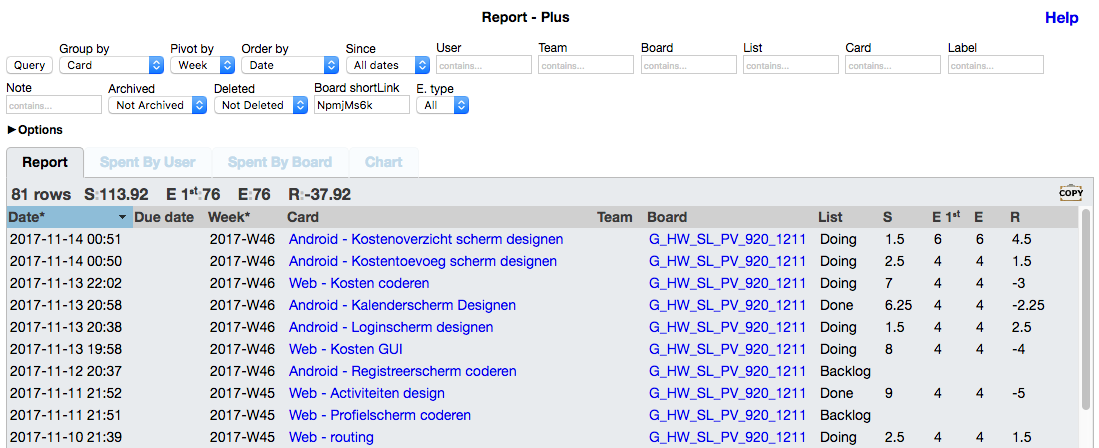
\includegraphics[width=\textwidth]{./afbeeldingen/individueleprestaties.png}
	\caption{Voorbeeld van een lijst met individuele tijdsbesteding}
	\label{fig:individueleprestaties}	
\end{figure} 
Het tabblad ``Spent by user'' geeft je een totaal overzicht van gespendeerde uren per teamlid per week.
Het tabblad ``Spent by board' geeft je een totaal overzicht van gespendeerde uren per bord per week.

\section{Burn-down Chart}

De burn-down chart toont een visueel overzicht van de drie tijdseenheden (S, E en R) voor het huidige bord. Een goede burn-down chart zal er dan ook naar streven om het aantal E uren stabiel te houden gedurende de uitvoering. Deze inschatting begint namelijk bij de aanvang van de iteratie, of aanmaken van het bord, en zou in principe niet meer mogen wijzigen tijdens de uitvoering ervan. Ook worden er normaal gezien geen kaarten toegevoegd tijdens de gesloten iteraties (programmeren). Daarnast zou de burn-down chart dan ook beschikken over een constant dalende curve (R) en een constant stijgende curve (S). Dit zou beteken dat de taken op een evenredig tempo werden afgewerkt waarbij het restrerende aantal uren op het einde van de sprint de 0 benadert.
\\\\
Om de burn-down chart van een bord te kunnen raadplegen gebruiken we de ``report'' knop \korteverwijzing[fig:burndownknop]. 
\begin{figure}[h]
	\centering
	
\includegraphics[scale=0.5]{./afbeeldingen/burndownknop.png}
	\caption{Genereren burn-down chart}
	\label{fig:burndownknop}	
\end{figure} 
\noindent
\\Op het scherm met de effectieve burn-down chart \korteverwijzing[fig:burndownchart] heb je naast de algemene grafiek ook nog de mogelijkheid om deze te verfijnen. Zo kan je de getoonde uren filteren (``View Filter'') of een overzicht raadplegen per gebruiker van zijn S, E en R uren (``View by user''). Daarnaast kan je ook inzoomen op de algemene grafiek door gebruik te maken van het muiswiel.

\begin{figure}[H]
	\centering
	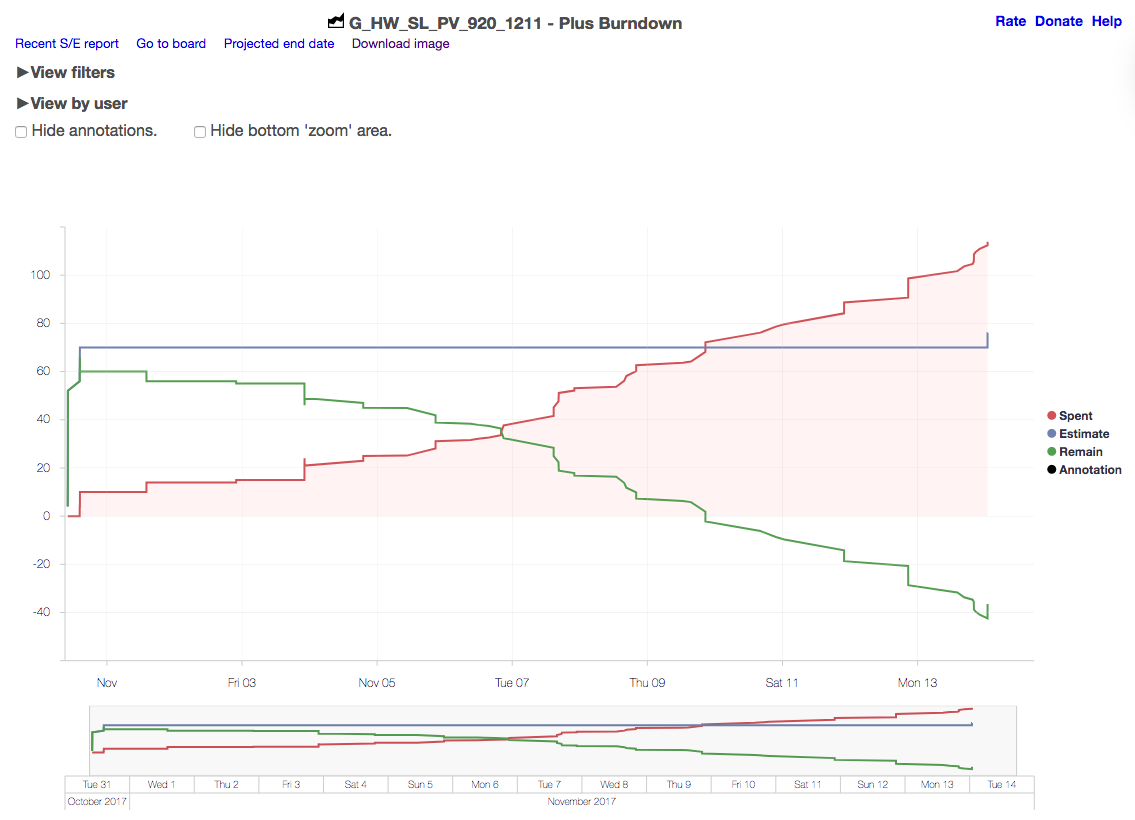
\includegraphics[scale=0.26]{./afbeeldingen/burndownchart.png}
	\caption{Voorbeeld van burn-down chart}
	\label{fig:burndownchart}	
\end{figure} 	
	\chapter{Uitbreidingen}

\section{GIT}

TODO: integratie met GIT	
\end{document}